\begin{frame}{Currently existing \gls*{inp} solutions}
    % \begin{table}[]
    %     \begin{tabular}{|r|l|}
    %     \hline
    %     Name      & Type                      \\ \hline
    %     IncBricks & In-network caching system \\ \hline
    %     NetChain  & Coordination services     \\ \hline
    %     Daiet     & In-network aggregation    \\ \hline
    %     SHArP     & Aggregation protocol      \\ \hline
    %     \end{tabular}
    % \end{table}
    \begin{enumerate}
        \item IncBricks (In-network caching system) % \cite{incbricks}
        \item NetChain (Coordination services) % \cite{netchain}
        \item Daiet (In-network aggregation) % \cite{daiet}
        \item SHArP (Aggregation protocol) % \cite{sharp}
    \end{enumerate}
\end{frame}

\begin{frame}{In-network caching system: IncBricks}
    % \begin{itemize}
    %   \item Custom fabric \textit{IncBox} (programmable switch + network accelerator)
    % \end{itemize}
    \centering
    \includegraphics[page=1, clip, trim=3.6cm 0.7cm 2.5cm 3.75cm, width=\textwidth]{analysis/inp/solutions.pdf}
\end{frame}

\begin{frame}{In-network caching system: IncBricks}
    \centering
    \includegraphics[page=2, clip, trim=3.6cm 0.7cm 2.5cm 3.75cm, width=\textwidth]{analysis/inp/solutions.pdf}
\end{frame}

\begin{frame}{In-network caching system: IncBricks}
    \centering
    \includegraphics[page=3, clip, trim=3.6cm 0.7cm 2.5cm 3.75cm, width=\textwidth]{analysis/inp/solutions.pdf}
\end{frame}

\begin{frame}{Coordination services: NetChain}
    \centering
    \includegraphics[page=6, clip, trim=3.6cm 0.7cm 3.2cm 4cm, width=\textwidth]{analysis/inp/solutions.pdf}
\end{frame}

\begin{frame}{In-network aggregation: Daiet}
    % Daiet \cite{daiet} is a system that performs in-network data aggregation for partition\hyp{}aggregate data center applications (big data analysis such as MapReduce \cite{mapreduce}, machine learning, graph processing, and stream processing). Inventors claim to achieve an 86.9\%-89.3\% traffic reduction, causing the execution time at the reducer to drop by 83.6\% on average.
    \centering
    \includegraphics[page=10, clip, trim=0.5cm 0.7cm 1.2cm 2.6cm, width=\textwidth]{analysis/inp/solutions.pdf}
\end{frame}

\begin{frame}{In-network aggregation: Daiet}
    \centering
    \includegraphics[page=11, clip, trim=0.35cm 0.6cm 0.3cm 2.6cm, width=\textwidth]{analysis/inp/solutions.pdf}
\end{frame}

\begin{frame}{Aggregation protocol: SHArP}
    \centering
    \includegraphics[page=15, clip, trim=3.3cm 0.9cm 1.6cm 3.4cm, width=\textwidth]{analysis/inp/solutions.pdf}
\end{frame}

\begin{frame}{Resource models (3.4)}
    \begin{columns}[T,onlytextwidth]
        \column{0.4\textwidth}
        \begin{enumerate}
            \item \glsentryfull{vc}\\
            \vspace{1mm}
            \begin{center}
                \includegraphics[page=1, clip, trim=0.5cm 0.6cm 3.85cm 1cm, width=0.7\textwidth]{analysis/models/solutions.pdf}
            \end{center}
            \item \glsentryfull{voc}
            \begin{itemize}
                \item $N$ \glsentryshortpl{vc} connected to a single root virtual switch
            \end{itemize}
            % \begin{center}
            %   \includegraphics[page=2, clip, trim=0.5cm 0.6cm 0.5cm 0.7cm, width=\textwidth]{analysis/models/solutions.pdf}
            % \end{center}
        \end{enumerate}
        \column{0.6\textwidth}
        \begin{enumerate}
            \setcounter{enumi}{2}
            \item \glsentryfull{tag}\\
            \begin{center}
                \includegraphics[page=3, clip, trim=0.5cm 0.5cm 0.5cm 0.5cm, width=0.95\textwidth]{analysis/models/solutions.pdf}
            \end{center}
            \item Fine-grained resource requests
            \begin{itemize}
                \item List of server-only resource demands
            \end{itemize}
            \item High-level goals
            \begin{itemize}
                \item E.g., job completion time (Bazaar \cite{bazaar})
            \end{itemize}
        \end{enumerate}
    \end{columns}
\end{frame}

% \begin{frame}{Intregrating INP resources in RMs}
% (3.3)
% \end{frame}

\begin{frame}{Level of network awareness in RMs}
    % 3.3.2
    \vspace{2mm}
    \begin{itemize}
        \item \glsentryshortpl{vm} proximity-aware
        \begin{itemize}
            \item Spreading \glsentryshortpl{vm} across different failure domains (e.g., racks, power domains, etc.)
            \item Omega \cite{omega}, \glsdesc{yarn}, Mesos \cite{mesos}, etc.
        \end{itemize}
        \item Bandwidth-aware
        \begin{itemize}
            \item Allowing tenants to specify bandwidth demands
            \item "Virtual network" models (i.e., \glsentryshortpl{vc}, \glsentryshortpl{voc} and \glsentryshortpl{tag})
            \item CloudMirror \cite{cloudmirror}, Oktopus \cite{oktopus}, Kraken \cite{kraken}, Proteus \cite{proteus}, etc.
        \end{itemize}
        \item Network resources-aware
        \begin{itemize}
            \item At the time of writing, there seemed to be only one embedding solution\footnote{\tiny{Rabbani, Md Golam, et al. "On tackling virtual data center embedding problem." \textit{2013 IFIP/IEEE International Symposium on Integrated Network Management (IM 2013)}. IEEE, 2013. \cite{ontackling}}} considering switch resources
            \item The scheduler places server and switch resources in separate rounds
        \end{itemize}
    \end{itemize}
    \vspace{5mm}
\end{frame}

% \begin{frame}{the only “network-aware” RM + its problems}
%   (3.3.2)
% \end{frame}
